% sections/titlepage.tex
% Esto asegura que la imagen de fondo se aplique solo a esta página de título
\thispagestyle{empty} % No mostrar número de página en la portada

% --- CONTENIDO DE LA PORTADA ---
\begin{titlepage}

    % Comando para añadir contenido al fondo de la página actual
    \AddToShipoutPictureBG{%
        \AtPageLowerLeft{%
            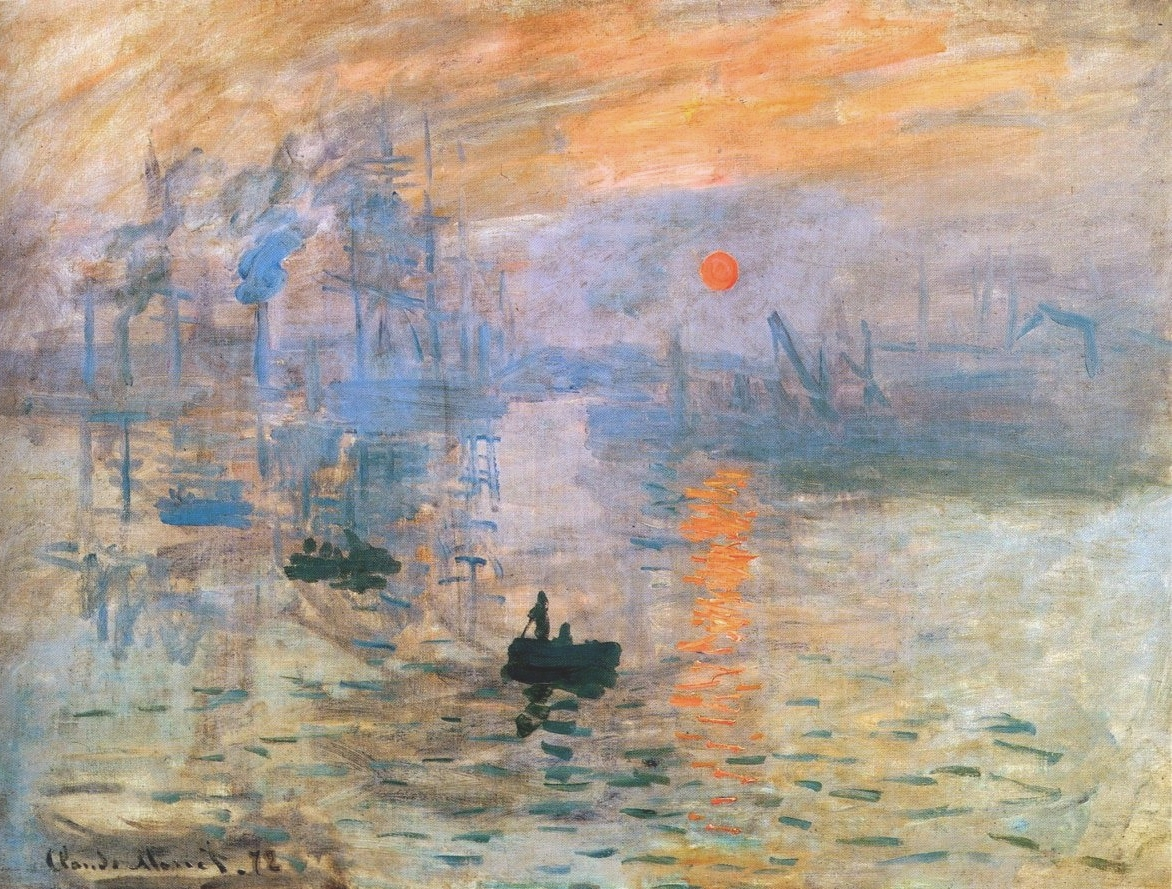
\includegraphics[width=\paperwidth,height=\paperheight]{images/background_image.jpg}% ¡Asegúrate de que este es el nombre correcto de tu imagen!
        }%
    }

    \centering % Centra todo el contenido de la portada

    \vspace*{1.5in} % Ajusta el espacio desde la parte superior (probablemente un poco más que 1in)

    % Título de la tesis: Más grande, negrita y mayúsculas
    {\fontsize{30}{35}\selectfont \textbf{\thesisTitle}} \par
    \vspace{1cm} % Espacio después del título (ajustado de 1.5cm a 1cm)

    % Autor: Grande
    {\Large \authorName} \par
    \vspace{0.7cm} % Espacio después del autor (ajustado de 1cm a 0.7cm)

    % Asesor: Tamaño normal
    {\large Advisor} \par
    {\advisorName} \par  
    \vspace{0.7cm} % Espacio después del asesor (ajustado de 1cm a 0.7cm)

    % Master Thesis
    {\large Master Thesis} \par
    \vspace{0.3cm} % Espacio más pequeño

    % Grado obtenido
    {\large Dissertation presented for the degree of\\ \degreeGranted} \par
    \vspace{0.3cm} % Espacio más pequeño

    % Materia
    {\large In the subject of\\ \subjectField} \par

    \vfill % Empuja la información de la universidad hacia la parte inferior

    % Información de la universidad: Mantenemos el mismo tamaño
    {\large \departmentName \\ \facultyName \\ \universityName} \par
    \vspace{0.5cm} % Espacio después de la universidad (mantenido)

    % Fecha: Mantenemos el mismo tamaño
    {\large \thesisDate} \par
    \vspace{0.5cm} % Espacio después de la fecha para que no quede pegada al borde

\end{titlepage}

\ClearShipoutPictureBG % Limpia el fondo para las páginas siguientes
\clearpage % Fuerza una nueva página